%%%%%%%%%%%%%%%%%%%%%%%%%%%%%%%%%%%%%%%%%
% kaobook
% LaTeX Template
% Version 1.2 (4/1/2020)
%
% This template originates from:
% https://www.LaTeXTemplates.com
%
% For the latest template development version and to make contributions:
% https://github.com/fmarotta/kaobook
%
% Authors:
% Federico Marotta (federicomarotta@mail.com)
% Based on the doctoral thesis of Ken Arroyo Ohori (https://3d.bk.tudelft.nl/ken/en)
% and on the Tufte-LaTeX class.
% Modified for LaTeX Templates by Vel (vel@latextemplates.com)
%
% License:
% CC0 1.0 Universal (see included MANIFEST.md file)
%
%%%%%%%%%%%%%%%%%%%%%%%%%%%%%%%%%%%%%%%%%

%----------------------------------------------------------------------------------------
%	PACKAGES AND OTHER DOCUMENT CONFIGURATIONS
%----------------------------------------------------------------------------------------

\documentclass[
	fontsize=12pt, % Base font size
	twoside=false, % Use different layouts for even and odd pages (in particular, if twoside=true, the margin column will be always on the outside)
	%open=any, % If twoside=true, uncomment this to force new chapters to start on any page, not only on right (odd) pages
	%chapterprefix=true, % Uncomment to use the word "Chapter" before chapter numbers everywhere they appear
	%chapterentrydots=true, % Uncomment to output dots from the chapter name to the page number in the table of contents
	numbers=noenddot, % Comment to output dots after chapter numbers; the most common values for this option are: enddot, noenddot and auto (see the KOMAScript documentation for an in-depth explanation)
	%draft=true, % If uncommented, rulers will be added in the header and footer
	%overfullrule=true, % If uncommented, overly long lines will be marked by a black box; useful for correcting spacing problems
]{kaobook}

% Set the language
%\usepackage[english]{babel} % Load characters and hyphenation
\usepackage[spanish]{babel}
\usepackage[english=british]{csquotes} % English quotes

% Load packages for testing
\usepackage{blindtext}
%\usepackage{showframe} % Uncomment to show boxes around the text area, margin, header and footer
%\usepackage{showlabels} % Uncomment to output the content of \label commands to the document where they are used

% Load the bibliography package
\usepackage{styles/kaobiblio}
%\usepackage[babel]{csquotes}
%\usepackage[style=apa,backend=biber]{biblatex}
%\DeclareLanguageMapping{spanish}{spanish-apa}
\addbibresource{main.bib} % Bibliography file

% Load mathematical packages for theorems and related environments. NOTE: choose only one between 'mdftheorems' and 'plaintheorems'.
\usepackage{styles/mdftheorems}
%\usepackage{styles/plaintheorems}

\usepackage{tikz}

 

\graphicspath{{examples/documentation/images/}{images/}} % Paths in which to look for images

\makeindex[columns=3, title=\'Indice Alfab\'etico, intoc] % Make LaTeX produce the files required to compile the index

%%\makeglossaries % Make LaTeX produce the files required to compile the glossary

\makenomenclature % Make LaTeX produce the files required to compile the nomenclature

% Reset sidenote counter at chapters
%\counterwithin*{sidenote}{chapter}

%----------------------------------------------------------------------------------------

\begin{document}

%----------------------------------------------------------------------------------------
%	BOOK INFORMATION
%----------------------------------------------------------------------------------------
%%%%%%%%%%%%%%%%%%%%%%%%%%%%
 
%\AddToShipoutPicture*{\BackgroundPic}     %%% background

\begingroup
\thispagestyle{empty} % Suppress headers and footers on the title page
\begin{tikzpicture}[remember picture,overlay]
	\node[inner sep=0pt] (background) at (current page.center) {\includegraphics[width=\paperwidth]{gid-3-org}};
  
  	\draw (current page.center) node [fill=yellow!30!white,fill opacity=0.6,text opacity=1,inner sep=1cm]{\Huge\centering\bfseries\sffamily\parbox[c][][t]{\paperwidth}{\centering Gestión de Información Documental\\[15pt] % Book title
		{\Large  Gu\'ia de Apoyo al curso de Gesti\'on de Informaci\'on Documental }\\[20pt] % Subtitle
		{\huge Dra. Virginia Padilla Sifontes}}}; % Author name
\end{tikzpicture}
\vfill
\endgroup

%%%%%%%%%%%%%%%%%%%%%%%%%%%%%%%%%

%----------------------------------------------------------------------------------------

\frontmatter % Denotes the start of the pre-document content, uses roman numerals

%----------------------------------------------------------------------------------------
%	OPENING PAGE
%----------------------------------------------------------------------------------------
 
%----------------------------------------------------------------------------------------
%	COPYRIGHT PAGE
%----------------------------------------------------------------------------------------
%%%%%%%%%%%%%%%%%%%%%%%%%%%%%%%%%%%%%%%%   VPVPVP

%----------------------------------------------------------------------------------------
%	COPYRIGHT PAGE
%----------------------------------------------------------------------------------------

\newpage
~\vfill
\thispagestyle{empty}

%\noindent Copyright \copyright\ 2021 Virginia Padilla\\ % Copyright notice

\noindent \textsc{Publicado por Virginia Padilla}\\ % Publisher

\noindent \textsc{\textbf{Declaraci\'on}\\
	Las figuras de las portadas y  encabezados de los cap\'itulos fueron elaborados por Andrea Isabel Revilla. \\ {en Instagram:  @ave.rebel \\ Twitter: @AveRebel \\ ArtStation \href{https://linktr.ee/avebel}{avebel} }  \\ Gracias Andrea Isabel!}\\ 

\noindent \textsc{ {Colof\'on} \\
	Este documento fue escrito con la ayuda de \href{https://sourceforge.net/projects/koma-script/}{\KOMAScript}  \href{https://www.latex-project.org/}{\LaTeX} usando la clase \href{https://github.com/fmarotta/kaobook/}{kaobook}.}

\noindent \textit{Primera Impresi\'on, Mayo 2021} % Printing/edition date

\noindent \textsc{ \textbf{Licencia} \\
 Este libro está licenciado bajo la licencia \href{http://creativecommons.org/licenses/by-sa/4.0/}{Creative Commons Atribución-CompartirIgual 4.0 Internacional.} 
} 

											


\includegraphics[width=0.4\linewidth]{by-sa.png}

%%%%%%%%%%%%%%%%%%%%%%%%%%%%%%%%%%%%%%

\makeatletter
\uppertitleback{\@titlehead} % Header



%\makeatother

%----------------------------------------------------------------------------------------
%	DEDICATION
%----------------------------------------------------------------------------------------
\newpage
\vspace*{\fill}
%\thispagestyle{empty}

%  {
 	
% 	\begin{flushright}
%	\Large {\textit{The harmony of the world is made manifest in Form and Number, and the heart and soul and all the poetry of Natural Philosophy are embodied in the concept of mathematical beauty.}\\
%	\flushright -- D'Arcy Wentworth Thompson
%4 4}
% \end{flushright}

%\vspace*{\fill}


%----------------------------------------------------------------------------------------
%	OUTPUT TITLE PAGE AND PREVIOUS
%----------------------------------------------------------------------------------------

% Note that \maketitle outputs the pages before here

% If twoside=false, \uppertitleback and \lowertitleback are not printed
% To overcome this issue, we set twoside=semi just before printing the title pages, and set it back to false just after the title pages
\KOMAoptions{twoside=semi}
%\maketitle
\KOMAoptions{twoside=false}

%----------------------------------------------------------------------------------------
%	PREFACE
%----------------------------------------------------------------------------------------

%\input{chapters/preface.tex}

%----------------------------------------------------------------------------------------
%	TABLE OF CONTENTS & LIST OF FIGURES/TABLES
%----------------------------------------------------------------------------------------

\begingroup % Local scope for the following commands

% Define the style for the TOC, LOF, and LOT
%\setstretch{1} % Uncomment to modify line spacing in the ToC
\hypersetup{linkcolor=blue} % Uncomment to set the colour of links in the ToC
\setlength{\textheight}{23cm} % Manually adjust the height of the ToC pages

% Turn on compatibility mode for the etoc package
\etocstandarddisplaystyle % "toc display" as if etoc was not loaded
\etocstandardlines % toc lines as if etoc was not loaded

\tableofcontents % Output the table of contents

\listoffigures % Output the list of figures

% Comment both of the following lines to have the LOF and the LOT on different pages
%\let\cleardoublepage\bigskip
%\let\clearpage\bigskip

\listoftables % Output the list of tables

\endgroup

%%%%%%% agreagado VP
%%%%%%%%%%%%%%%%%%%%%
\newcommand{\li}{\textit{LI}\xspace}   
\newcommand{\nr}{\textit{NR}\xspace}   
\newcommand{\pa}{\textit{PA}\xspace}   
\newcommand{\ka}{\textit{KA}\xspace}   
\newcommand{\gu}{\textit{GU}\xspace}  
\newcommand{\av}{\textit{AV}\xspace}    
 
\newcommand{\LI}{\textit{Universidad Pedag\'ogica Experimental Libertador, (2011). Manual de trabajos de grado y especializaci\'on y maestr\'ia y tesis doctorales.}\xspace}
\newcommand{\NR}{\textit{Naranjo, E.(2010). Uso de los sistemas de informaci\'on documental en la educaci\'on superior: estado del arte}\xspace}
\newcommand{\PA}{\textit{Paiva, A.(2007). A internet na forma{\c c}{\~a}o inicial de professores: um estudo em pesquisa de informa{\c c}{\~a}o (Disserta{\c c}{\~a}o de Mestrado em Comunica{\c c}{\~a}o Educacional Multimedia)}\xspace}
\newcommand{\KA}{\textit{Kaushik, A.(2012). Avalia{\c c}{\~a} de recursos da internet: uma revis{\c c}{\~a}o de literatura selecionada}\xspace}
\newcommand{\GU}{\textit{Guirao-Goris y otros (2008). El art\'iculo de revisi\'on}\xspace}
\newcommand{\AV}{\textit{Avello, R  y otros (2013). Zotero, más allá de un gestor bibliográfico: Una experiencia con los docentes y nuevas metas.}\xspace}


% Prints the month name (e.g., January) and the year (e.g., 2008)
%%\newcommand{\monthyear}{%
%%	\ifcase\month\or Enero\or Febrero\or Marzo\or Abril\or Mayo\or Junio\or  Julio\or Agosto\or Septiembre\or Octubre\or Noviembre\or   Diciembre\fi\space\number\year  }

%%%%%%%%%   VP

%----------------------------------------------------------------------------------------
%	MAIN BODY
%----------------------------------------------------------------------------------------

\mainmatter % Denotes the start of the main document content, resets page numbering and uses arabic numbers
\setchapterstyle{kao} % Choose the default chapter heading style



\setchapterpreamble[u]{\margintoc}
\setchapterimage{gid-3-org}
%\setchapterpreamble[u]{\margintoc}

\chapter*{Introducci\'on}
 
\labch{intro}

%%\section{The Main Ideas}

El objetivo de este  documento es que sirva de gu\'ia de apoyo para el  curso Gestión de Información Documental, asignatura introductoria  del Postgrado de Finanzas de la Universidad Nacional Experimental de Guayana. 

El propósito de la asignatura Gesti\'on de la Informaci\'on Documental es que el participante conozca cómo  formular estrategias de búsqueda y recuperación de información, evaluar la confiabilidad de las fuentes de información disponibles y construir una base de datos personal con el apoyo de un gestor bibliográfico que permita su registro sistemático y comunicación en el\href{https://normasapa.com/normas-apa-2019-cuestiones-mas-frecuentes/comment-page-11/}{ estilo APA}. 

La asignatura se dicta a trav\'es  del aula virtual \href{http://moodle.uneg.edu.ve/moodle/}{Gesti\'on de Informaci\'on Documental} construida bajo la plataforma de aprendizaje en l\'inea  \href{https://moodle.org/?lang=es}{Moodle} de la Universidad Nacional Experimental de Guayana.



El presente documento esta estructurado en cuatro cap\'itulo que corresponde con las secciones que conforman el aula virtual del curso. A saber:
\begin{description}
	\item [Revisi\'on Documental.] Se define la Revisi\'on Documental y se exponen los tipos de revisiones que se pueden elaborar.

	\item [Metodolog\'ia de la Revisi\'on Documental.] La metodolog\'ia para la revisi\'on documental se inicia en esta sesi\'on con la construcci\'on de las cadenas de b\'usqueda de informaci\'on; adem\'as de, la escogencia de la fuentes de informaci\'on.

	\item [Organizaci\'on Informaci\'on Documental.] En esta sesi\'on se presentan las t\'ecnicas y criterios para organizar y seleccionar los documentos relevantes a la revisi\'on que se va a hacer.

	\item [Redacci\'on del Documento de Revisi\'on.] Se presentan los criterios para una redacci\'on fluida y clara.
	
\end{description}


Las figuras de las portadas y  encabezados de los cap\'itulos fueron elaborados por Andrea Isabel Revilla. Pueden ver su portafolio  en Instagram:  @ave.rebel \\ Twitter: @AveRebel \\ ArtStation \href{https://linktr.ee/avebel}{avebel} . Gracias Andrea Isabel! 

Este documento fue escrito con la ayuda de \href{https://sourceforge.net/projects/koma-script/}{\KOMAScript}  \href{https://www.latex-project.org/}{\LaTeX} usando la clase \href{https://github.com/fmarotta/kaobook/}{kaobook}.

Para la redacci\'on del documento se usan las normas de estilo de la \href{https://uc3m.libguides.com/guias_tematicas/citas_bibliograficas/estilo-ieee}{IEEE}.

Cualquier error u omisi\'on es de mi absoluta responsabilidad. Agradezco que env\'ien su  comentarios, observaciones o quejas a la direcci\'on electr\'onica virginiapadillas@gmail.com.





\pagelayout{wide} % No margins
%%\addpart{Class Options, Commands and Environments}
\pagelayout{margin} % Restore margins

\input{chapters/1-definicion.tex}
\setchapterstyle{kao}

\setchapterimage[6cm]{gid-3-org}
\setchapterpreamble[u]{\margintoc}

\chapter{Metodolog\'ia de Revisi\'on Documental }
\label{ch:met-RevDoc}
\index{revisi\'on documental!metodolg\'ia}

       En esta parte se presenta la metodología para la revisión documental. La metodología se presenta en dos fases :  \index{metodolog\'ia!dise\~no de la b\'usqueda}
		\index{metodolog\'ia!an\'alisis cr\'itico}

\begin{itemize}
	\item Diseño de la Búsqueda. Esta fase es la que se detalla en este cap\'itulo. Consta de los siguientes pasos:  
	\begin{description}
		\item Definición de Descriptores
		\item Uso de Tesauros
		\item Estrategias de búsquedas
		\item Diseño de la búsqueda
		\item Bases de Datos para la búsqueda
	\end{description}
	\item Análisis Crítico de Documentos. En esta fase se completa la metodolog\'ia de revisi\'on documental
	\begin{description}
		\item Organización de la información acopiada
		\item Criterio de selección de documentos
		\item Resultados de la búsqueda
	\end{description}
\end{itemize} 

\begin{marginfigure}[-3cm]%
	\includegraphics[width=\linewidth]{imagen1}
	%	\caption{Fichas bibliogr\'aficas }
	%	\label{fig:Fichas}
\end{marginfigure} 

Ejemplificaremos la metodología mediante el planteamiento de dos pesquisas. La primera pregunta de  investigación planteada en  \sidecite{Naranjo2010}:
 ?` Los Sistemas de Información Documental, en tanto medios, cómo posibilitarían la estructuración de los datos y la información en conocimiento con fines formativos en la educación superior ?

La segunda es una investigación dirigida a conocer  como evaluar recursos de internet "necesidad de evaluación de los recursos de Internet"; "Preocupación del bibliotecario por los recursos de evaluación"; y "Criterios para evaluar diferentes recursos de Internet",  que se presenta en  \sidecite{Kaushik2012}.

\section{ Definición de Descriptores}

\index{b\'usqueda de informaci\'on!tesauro} 

  Los descriptores o palabras claves  establecen un vocabulario controlado o los temas que  trata  un texto. En una pregunta o preguntas de investigación, definen las áreas de conocimientos  que se deben explorar para un búsqueda de documentos.
  
  En la pregunta de investigación que se usan como ejemplo para ilustrar este concepto: 
  
  \begin{marginfigure}[-3.3cm]%
  	\includegraphics[width=\linewidth]{KeyW}
  	%	\caption{Fichas bibliogr\'aficas }
  	%	\label{fig:Fichas}
  \end{marginfigure}
  
  
   ?` Los Sistemas de Información Documental, en tanto medios, cómo posibilitarían la estructuración de los datos y la información en conocimiento con fines formativos en la educación superior?    
  se infiere que los descriptores son los siguientes: 
  
  \begin{marginfigure}[-3cm]%
  	\includegraphics[width=\linewidth]{keyW}
  	%	\caption{Fichas bibliogr\'aficas }
  	%	\label{fig:Fichas}
  \end{marginfigure}
  
  	\marginnote[-4.2cm]{
  	\begin{kaobox}[frametitle= Palabras de b\'usqueda ]
  		\begin{description}
  			\item[Sistema de información \\ documental] 
  			\item[Dato] 
  			\item[Información] 
  			\item[Conocimiento] 
  			\item[Sistema didáctico] 
  			\item[Información] 
  			\item[Estrategia didáctica] 
  		\end{description}
  		
  	\end{kaobox}
  } 
  
 
  En la  investigación dirigida a conocer a conocer como evaluar recursos de internet "necesidad de evaluación de los recursos de Internet"; "Preocupación del bibliotecario por los recursos de evaluación"; y "Criterios para evaluar diferentes recursos de Internet", las palabras de  búsquedas son:
   
   	\marginnote[-2.2cm]{
   	\begin{kaobox}[frametitle= Palabras de b\'usqueda]
   		\begin{description}
   			\item[recursos de internet] 
   			\item[evaluar] 
   			\item[criterios de evaluación] 
   			\item[bibliotecario]  
   		\end{description}
   		
   	\end{kaobox}
   } 
   
    \begin{kaobox}[frametitle=Ejercicio]
    	Establezca una pregunta o preguntas de investigación que direccionen una revisión bibliográfica. Defina las palabras claves.
    \end{kaobox}

\begin{marginfigure}[-1.2cm]%
	\includegraphics[width=\linewidth]{pregunta}
	%	\caption{Fichas bibliogr\'aficas }
	%	\label{fig:Fichas}
\end{marginfigure}

\section{Consulta de tesauro}

El propósito de consultar un tesauro es conocer, además de la definición del término, los sinónimos, antónimos y la jerarquía de palabras o palabras derivadas del término buscado.

\index{b\'usqueda de informaci\'on!tesauro}
 
 
 	\marginnote[-3.2cm]{
	\begin{kaobox}[frametitle= Tesauro]

		El Tesauro  es una lista controlada y estructurada de términos para el análisis temático y la búsqueda de documentos y publicaciones en los campos de la educación, cultura, ciencias naturales, ciencias sociales y humanas, comunicación e información  
			
	\end{kaobox}
} 

Una busqueda del t\'ermino \textins{tesauros en l\'inea} con su buscador en la red, le muestra un conjunto de tesauros disponibles que puede usar. 
\index{b\'usqueda de informaci\'on!tesauro en l\'inea}


	\marginnote {
	\begin{kaobox}[frametitle= Tesauros en Finanzas]	
			En este enlace puede consultar el tesuaro  del \'area de  	\href{http://vocabularies.unesco.org/browser/thesaurus/es/page/concept663}{Tesauro de finanzas}  
		
 
	\end{kaobox}
} 

La consulta en tesauros (por ejemplo, usaremos el tesauro de la UNESCO) acerca de palabras relacionadas a las palabras claves, arrojan solo sinónimos para el primer término, en la consulta de \sidecite{Naranjo2010}: 



\begin{description}
	\item[Sistema de información documental] servicio bibliográfico, biblioteca
	\item [Dato]
	\item [Información]
	\item [Conocimiento]
	\item [Sistema didáctico]
	\item [Estrategia didáctica ]
\end{description}


Para la investigación establecida por \sidecite{Kaushik2012}: 


\begin{description}
	\item [recursos de internet:]  fuentes de internet
	\item [evaluación:]  medición
	\item [criterios de evaluación]
	\item [bibliotecario ]
\end{description}

 

Ademas de las palabras relacionadas, los conceptos plasmados en el tesauro se incluyen  en el documento cuando define el problema de su investigación  o el área de su estudio.

\begin{marginfigure}[1.2cm]%
	\includegraphics[width=\linewidth]{pregunta}
	%	\caption{Fichas bibliogr\'aficas }
	%	\label{fig:Fichas}
\end{marginfigure}
\section{Establecer las estrategias de búsquedas}

 \begin{kaobox}[frametitle= Ejercicio ]
Explore la internet usando su buscador de preferencia, explore los tesauros disponibles. Elija los que va a usar como fuente de información y busque las palabras relacionadas y los conceptos concernientes a las palabras claves de su investigación. Use Zotero o el gestor de documento preferido para capturar esas fuentes de datos. Indique en su respuesta: Tesauro usado en formato de normas APA. Si usa el gestor de documento, solo cópielo de se bibliografía. Resultado de las consultas en el tesauro: palabras relacionadas y conceptos asociados a las palabras claves  	
 \end{kaobox}


\begin{marginfigure}[-2cm]
	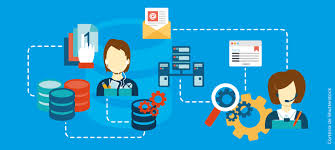
\includegraphics[width=\linewidth]{criterio}
	%	\caption{Fichas bibliogr\'aficas }
	%	\label{fig:Fichas}
\end{marginfigure}

Se arman las búsquedas en la biblioteca estableciendo las cadenas de búsquedas. La estrategia para armar estas cadenas es combinar las palabras claves usando los conectores booleanos or, and, not. 
  
Las cadenas de búsquedas van a ser usadas como entrada en los buscadores de documentos. Note las asociaciones de las claves expresadas por medio de paréntesis. 
Por ejemplo:
(Sistema de información documental \textbf{or} servicio bibliográfico \textbf{or} biblioteca )  se agruparon de esta manera ya que son términos homónimos.
((dato) \textbf{or} (información) \textbf{or} (conocimiento) )  a pesar de tener distintas acepciones,  se buscarán documentos que tengan cualquiera de esas palabras

\begin{marginfigure}[-2.2cm]
	\includegraphics[width=\linewidth]{imagen3}
	%	\caption{Fichas bibliogr\'aficas }
	%	\label{fig:Fichas}
\end{marginfigure}

Las cadenas establecidas son:
\begin{itemize}
	\item (Sistema de información documental \textbf{or} servicio bibliográfico \textbf{or} biblioteca) \textbf{and} ((dato) \textbf{or} (información) \textbf{or} (conocimiento) ) \textbf{or} (Sistema didáctico ) \textbf{or}  (Estrategia didáctica)
	
	\item (Sistema de información documental \textbf{or} servicio bibliográfico \textbf{or} biblioteca) \textbf{and} (Sistema didáctico ) \textbf{not} (Estrategia didáctica) \textbf{or} ((dato) \textbf{or} (información) \textbf{or} (conocimiento) ) 
	
	\item (Sistema de información documental \textbf{or} servicio bibliográfico \textbf{or} biblioteca) \textbf{and} (Estrategia didáctica) \textbf{not} (Sistema didáctico )  \textbf{or} ((dato) \textbf{or} (información) \textbf{or} (conocimiento) ) 
\end{itemize}

 \begin{marginfigure}[-1.2cm]%
 	\includegraphics[width=\linewidth]{pregunta}
 	%	\caption{Fichas bibliogr\'aficas }
 	%	\label{fig:Fichas}
 \end{marginfigure}

\begin{kaobox}[frametitle= Ejercicio]
Indique las cuales serían las cadenas de búsqueda que usaría para su recolección de investigación. 	
\end{kaobox}


 
 \section{Base de Datos para la búsqueda}

\index{b\'usqueda de informaci\'on!base de datos}                 
 La búsqueda de la literatura para elaborar un artículo de revisión se puede realizar en varios tipos de fuentes de información. Existen diferentes clasificaciones de los tipos de documentos que podemos manejar en nuestra búsqueda bibliográfica. \sidecite{Paiva2007}
 Una de las más utilizadas es aquella que distingue entre tipos de documentos provenientes de:
 

 
 \begin{description}  
 	\index{b\'usqueda de informaci\'on!fuentes }
 	\item[Fuentes primarias.] Originales, transmiten información directa (artículos originales, tesis).
 	
 	\item[Fuentes secundarias.] Ofrecen descripciones de los documentos primarios (catálogos, bases de datos, revisiones sistemáticas, resúmenes). 
 	
 	\item[Fuentes Terciarias.] Sintetizan los documentos primarios y los secundarios (directorios).
 \end{description}
 
 Las bases de datos son una fuente secundaria de datos homogéneos recuperables a través de internet. Contienen registros o referencias bibliográficas completas de fuentes primarias (artículos de investigación, libros, tesis, entre otros), organizados en campos que cubren todos los aspectos de la información (título, autor, resumen, etc.)
 
  \begin{marginfigure}[-2cm]%
 	\includegraphics[width=\linewidth]{basedatos}
 	%	\caption{Fichas bibliogr\'aficas }
 	%	\label{fig:Fichas}
 \end{marginfigure}
 
 Establecer las bases de datos especializadas donde se van a extraer información. Ejemplos de estas bases de datos:
 
 \begin{marginfigure}[2cm]%
 	\includegraphics[width=\linewidth]{imagen2}
 	%	\caption{Fichas bibliogr\'aficas }
 	%	\label{fig:Fichas}
 \end{marginfigure}
 
 \begin{itemize}
 	\item  \href{https://www.ebsco.com/es/productos/bases-de-datos}{LISTA}: Library, Information Science \& Technology Abstracts. 
 	
 	\item \href{https://about.proquest.com/products-services/lisa-set-c.html}{LISA}: Library and Information Science Abstract.  
 	
 	\item  \href{https://libguides.du.edu/c.php?g=90436&p=582594}{ERICH}: Education Resources Information Center, H. W. Wilson and Emerald.   
 	 
 	\item   Motor de búsqueda \textbf{Google}, \textbf{Google Scholar},\textbf{CiteseerX}, \textbf{Science Direct}.
 	
  	\item  	Redalyc: Red de Revistas Científicas de América Latina y el Caribe
 \end{itemize}
   
 
 Las bases de datos seleccionadas para la búsqueda pueden presentarse en una tabla que sintetice esta colección. La estructura del cuadro \ref{tab:recursos} es la siguiente. Cada celda contiene información de un recurso:
 
  	\begin{table}[h] 
  	\footnotesize%
  	\begin{center}
  		\footnotesize
  		\begin{tabular}{|c|c|c|c|}
  			\hline
    		   Recurso &   \multicolumn{3}{|c|}{Nombres}  \\
  			\hline  			
  			\tiny{Bibliotecas Universitarias} &   &  &  \\
  				\hline  			
  		\tiny{Sitios Web} & \tiny{Google}  & \tiny{CieseerX} & \\
  			\hline  			
  		\tiny{Bases de Datos}  &  \tiny{Redalyc} &  & \\
  			\hline  			
  		\tiny{Revistas Electr\'onicas} &  \tiny{Strategos} & & \\
  			\hline  	  		
  		\end{tabular}
  	\end{center}
  	\caption{Recursos y Sistemas de Información }
  	\label{tab:recursos}
  \end{table}
  
 
  \begin{marginfigure}[1.2cm]%
 	\includegraphics[width=\linewidth]{pregunta}
 	%	\caption{Fichas bibliogr\'aficas }
 	%	\label{fig:Fichas}
 \end{marginfigure}
 
 
 \begin{kaobox} [frametitle= Ejercicio ]
 	Los artículos de revisión documental o estado del arte se basan en documentos provenientes de fuentes primarias. Indique cuales serían las bases de datos para la búsqueda de estos documentos.
 	Presente esas bases de datos en la tabla de Recursos y Sistemas de Información.
 	
 	\end{kaobox}
 

 
  
     




\setchapterstyle{kao}

\setchapterimage[6cm]{gid-3-org}
\setchapterpreamble[u]{\margintoc}

\chapter{Organización de información documental }
\label{ch:org-info}
\index{informaci\'on documental!organizaci\'on}

 Una vez que se recupera la información , se procede a valorarla; es decir, a analizar y evaluar su relevancia de acuerdo con el problema y la hipótesis de investigación. De cada uno de los documentos seleccionados, se conservan sus respectivas fichas bibliográficas referenciales. Toda esta información es recopilada con el gestor documental Zotero.
 
 \marginnote [1cm] {
 	\begin{kaobox}[frametitle= Zotero]
 		Zotero es una herramienta gratuita y fácil de usar que le ayuda a recopilar, organizar, citar y compartir investigaciones. Los siguientes son enlaces de ayuda:\\
 		\href{https://www.zotero.org/}{P\'agina de Zotero} 
 		\href{https://www.youtube.com/watch?v=7iz0lJLI5L4}{Zotero y Word}  y
 		\href{https://www.zotero.org/support/es/quick_start_guide}{Tutorial}
 	\end{kaobox}
 } 
 
 	\begin{marginfigure}[7cm]%
 		\includegraphics[width=\linewidth]{imagen2}
 	%	\caption{Fichas bibliogr\'aficas }
 	%	\label{fig:Fichas}
 	\end{marginfigure}
 
 	
 	
 
Las fichas bibliográficas contienen información acerca de:
 Datos relacionados con el tipo de publicación, ubicación e identificación del documento y las respectivas categorías de análisis. Se establece si es un artículo de revista, libro producto de investigación, capítulo de libro, trabajo de investigación, sistema de investigación, o evento (ponencia); además, si es una   investigación que forma parte de la educación formal como monografía, trabajo de investigación de maestría o tesis doctoral. 
 
 
 La ubicación del documento se refiere al lugar donde se encontró, esto es, en bases de datos, bibliotecas, archivo personal o un recurso Web; además, se aclara si el documento es en texto completo o referencial; el nombre del sistema en que se recuperó la información; si está en formato impreso o digital; la dirección electrónica y la fecha de consulta. 
 
 
 La identificación del documento se realiza a partir del título, del autor, del título de la publicación, del país (bien sea de la publicación o del autor, aquí no se discriminó), del idioma en que se encuentra el texto, del número de páginas y de las palabras clave que presenta la publicación.
 
 

\section{Criterios de selección de documentos}

 \index{documentos!criterios de selecci\'on}     
Los criterios de selección se encuentran determinados por los objetivos de la revisión, es decir la pregunta a la que trata de responder el artículo. Otro de los aspectos que determina la selección de los artículos es su calidad metodológica y si cumplen con los criterios de calidad científica buscada. En una primera fase los aspectos que deberemos tener en cuenta serán:  \textit{el título, los autores, el resumen} y\textit{ los resultados}.


\begin{marginfigure}[-3,2cm]%
	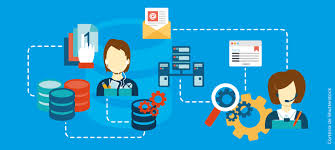
\includegraphics[width=\linewidth]{criterio}
	%	\caption{Fichas bibliogr\'aficas }
	%	\label{fig:Fichas}
\end{marginfigure}

Otros criterios que se podrían tener en cuenta son:  \textit{tipo de publicación , el título, los autores, el resumen} y \textit{los resultados, cantidad de citaciones}

Luego, se procede al análisis respectivo mediante una lectura crítica. La pagina \href{https://www.redcaspe.org/}{CASPe}  define la lectura crítica como una técnica que ofrece la oportunidad de aumentar la efectividad de nuestra lectura, adquiriendo las habilidades necesarias para excluir con la mayor prontitud los artículos científicos de mala calidad y aceptar aquellos otros con la suficiente calidad científica para ayudarnos en nuestra toma de decisiones para el cuidado de los pacientes. 

\begin{marginfigure}[-3.2cm]%
	
\includegraphics[width=\linewidth]{criterio2}
	%	\caption{Fichas bibliogr\'aficas }
	%	\label{fig:Fichas}
\end{marginfigure}

\begin{marginfigure}[3.2cm]%
	\includegraphics[width=\linewidth]{imagen1}
	%	\caption{Fichas bibliogr\'aficas }
	%	\label{fig:Fichas}
\end{marginfigure}



Proponen que los artículos científicos deben ser evaluados en tres aspectos: 


\begin{itemize}
	\item ?`Podemos confiar en los resultados? Dicho de otra forma:  ?`son válidos? Es decir,   enjuiciamos la validez metodológica del artículo.  Dependiendo de la validez de un artículo lo podemos clasificar dentro de una escala de niveles de evidencia y grados de recomendación. 

 	\item   ?`Cuáles son los resultados? Por ejemplo, ?`Sistema de información documental frente a Sistemas didáctico muestra alguna relación ?  ?`cómo miden esta relación ? ?`son precisos los resultados?

	\item ?`Son pertinentes o aplicables estos resultados en mi área ?
\end{itemize}


\begin{marginfigure}[1.2cm]%
	\includegraphics[width=\linewidth]{pregunta}
	%	\caption{Fichas bibliogr\'aficas }
	%	\label{fig:Fichas}
\end{marginfigure}

\begin{kaobox}[frametitle=Ejercicio]
	Establezca los criterios que va a usar para la revisi\'on de sus documentos. %%%%%
\end{kaobox}


%%%%%%%%%%%%%%%%
\section{Mapas para organizar documentos}
 \index{documentos!mapas para organizar}     

 No hay una organización establecida para los art\'iculos de investigaci\'on provenientes de una revisión documental. Por tanto, cada autor tendrá que elaborar la suya propia. La
regla fundamental para escribir un trabajo de esta clase es preparar un guión \cite{GuiraoGoris2008}.


\begin{marginfigure}[1cm]%
	\includegraphics[width=\linewidth]{mapaconceptual}
	%	\caption{Fichas bibliogr\'aficas }
	%	\label{fig:Fichas}
\end{marginfigure}
 Si la información esta bien organizada, cuenta con una estructura lógica que va introduciendo de forma secuencial y razonable la información, el artículo estará mejor redactado y permitirá una fácil lectura y comprensión. Por tanto, la elaboración de un guión es fundamental.
 
De acuerdo a \GU, la  metodología para la elaboración
de un guión tras una lectura crítica de los textos se basa en los siguientes pasos:  Ordenar, Rotular, Integrar, Priorizar. 


\begin{marginfigure}[2.2cm]%
	\includegraphics[width=\linewidth]{revision5}
	%	\caption{Fichas bibliogr\'aficas }
	%	\label{fig:Fichas}
\end{marginfigure}

\begin{description}
	\item[Ordenar:] Se reduce la información eliminando todo aquello que no es esencial mediante un proceso que pasa por segmentar la información básica. Ordenar dicha información por conjuntos, agrupando esta información esta comienza a adquirir  características comunes.
  
	\item[Rotular:] En esta fase se asigna un nombre a cada grupo. Si no es posible decidir el nombre, se puede asignar un código arbritario como una letra, color o número.
	
	\item[Integrar:]  Con los grupos ya formalizados y
	etiquetados se procede a integrar los grupos que se parezcan bastante, de forma que habrá algunos que queden aislados y otros integrados.  
	
	\item[Priorizar:] Tras estos procesos se priorizan los grupos para identificar la información que será más relevante dentro de la organización alcanzada.
\end{description}


\begin{marginfigure}[1cm]%
	\includegraphics[width=\linewidth]{mapamental2}
	%	\caption{Fichas bibliogr\'aficas }
	%	\label{fig:Fichas}
\end{marginfigure}
 
  
En este proceso de estructuración de los datos se puede recurrir a la realización de un mapa conceptual o un mapa mental según sea lo más apropiado. Se muestra la estructura de la informaci\'on en un mapa mental que se usa en el documento \GU ,  en la figura \ref{fig:mapa}

 


\begin{figure}%
	\includegraphics {MapaMental}
	\caption{Mapa Mental. Tomado de \GU }
	\label{fig:mapa}
\end{figure}

A medida que se localizan documentos, la información se va incluyendo en este esquema o percha de análisis de modo que tras haber realizado toda la lectura de la bibliografía y seleccionado la información más relevante se cuelga de cada percha o ítem. De esta manera se puede ir combinando la información de diferentes fuentes en una estructura de carácter común para iniciar la redacci\'on del artículo de revisi\'on. 
En la figura \ref{fig:percha} se ejemplifica cómo la información extraída de diferentes fuentes se organizó en cada ítem de la percha en el \GU.




\begin{figure}%
	\includegraphics[width=0.8\linewidth]{Percha}
		\caption{Percha de an\'alisis. Tomado de \GU }
		\label{fig:percha}
\end{figure}
 


%%%%


 \section{Resultados de la búsqueda}
 
  \index{documentos!resultados de la b\'usqueda}     
 
 Los resultados de la búsqueda y revisión, se puede presentar en el cuadro \ref{tab:resultados} donde por cada recurso se plasman los resultados parciales que representan la cantidad de documentos arrojados por la búsqueda. Y en resultados definitivos se colocan la cantidad de artículos que se seleccionaron una vez que se aplicó  el criterio de selección de documentos.
 
 \begin{marginfigure}[-3.2cm]%
 	\includegraphics[width=\linewidth]{imagen3}
 	%	\caption{Fichas bibliogr\'aficas }
 	%	\label{fig:Fichas}
 \end{marginfigure}
 


\begin{table}[h]\index{{recursos!resultados}}
	\footnotesize%
	\begin{center}
		\footnotesize
		\begin{tabular}{|c|c|c|}
			\hline
			 Recurso & Resultados Parciales & Resultados Definitivos  \\
			\hline  			
		 {LISTA} &   &  \\
		 \hline
		  {LISA} &   &  \\
		  \hline
		  Google Scholar &   &  \\
		  \hline
	         	  &   &  \\
	         	  \hline
	              &   &  \\
	              
			\hline  			
			
		\end{tabular}
	\end{center}
	\caption{Resultados por Recursos }
	\label{tab:resultados}
\end{table}


\begin{marginfigure}[-1.2cm]%
	\includegraphics[width=\linewidth]{pregunta}
	%	\caption{Fichas bibliogr\'aficas }
	%	\label{fig:Fichas}
\end{marginfigure}

\begin{kaobox}[frametitle=Ejercicio]

	 Una vez obtenido los resultados de su búsqueda en las bases de datos, coloque la cantidad de documentos arrojados por la búsqueda en  la columna\textit{ Resultados Parciales} de la tabla Resultados por Recursos.
	Note que puede ajustar o restringir este número, perfeccionando los criterios de búsqueda.
	Defina cu\'ales son los criterios de evaluación de documento que va a utilizar y aplíquelo a sus resultados parciales. Una vez finalizado, plasme en la columna \textit{Resultados Definitivos} de la ya mencionada tabla, la cantidad de documentos elegidos.
	Indique:
		\begin{itemize}
			\item ?`Que criterios de evaluación utilizó?
			\item  Llene la Tabla de Resultados por Recursos con sus resultados obtenidos.
			\item Presente mapa mental o conceptual con la  informaci\'on recolectada.
		\end{itemize}
	\end{kaobox}


\section{Bibliograf\'ia de la b\'usqueda}

 \index{documentos!bibliograf\'ia}     

El resultados de la selección de artículos conforma la bibliografía de su informe. Esta debe estar construida de acuerdo a las normas APA \sidecite{Libertador2011}  Al usar gestor de referencias bibliográficas  como Zotero, esta bibliografía se tiene disponible en este sistema normas. 



\begin{table}[h] 
	\footnotesize%
	\begin{center}
		\footnotesize
		\begin{tabular}{|c|c|}
			\hline
			\'Indice (autor (es), fecha) & Descripci\'on del documento     \\
			\hline  			
			  &    \\
			  \hline
			    &  \\
			    \hline
			   &  \\
			   \hline
		  &  \\
		 
			\hline  			
			
		\end{tabular}
	\end{center}
	\caption{Bibliograf\'ia }
	\label{tab:biblio}
\end{table} 


\begin{marginfigure}[1.2cm]%
	\includegraphics[width=\linewidth]{pregunta}
	%	\caption{Fichas bibliogr\'aficas }
	%	\label{fig:Fichas}
\end{marginfigure}

\begin{kaobox}[frametitle=Ejercicio]
	Plasme a continuación la bibliografía con sus artículos seleccionados y preséntela en la tabla \ref{tab:biblio}:
\end{kaobox}

 
\setchapterstyle{kao}

\setchapterimage[6cm]{gid-3-org}
\setchapterpreamble[u]{\margintoc}

\chapter{Redacción  del documento de revisión }
\label{ch:org-info}
\index{revisi\'on documental!redacci\'on de documentos}



 Redactar, etimológicamente significa compilar o poner en orden; en un sentido más preciso consiste en expresar por escrito los pensamientos o conocimientos ordenados con anterioridad. Para redactar un artículo de carácter científico  en el \GU  se  apunta las cualidades esenciales de un buen estilo: 
 
 \begin{marginfigure}[-1.2cm]%
 	\includegraphics[width=\linewidth]{revision4}
 	%	\caption{Fichas bibliogr\'aficas }
 	%	\label{fig:Fichas}
 \end{marginfigure}
 
 
 
 \begin{description}
 	\item [Claridad.] Se es claro cuando el escrito penetra sin esfuerzo en la mente del lector. Para lograr la claridad no basta tener las ideas claras. Es necesario que la construcción de la frase y el párrafo responda al orden lógico de las ideas. Para asegurar esto último es conveniente ligar las ideas entre dos o más frases. 
 	
 	\item[Concisión.] se es conciso cuando se usa sólo las palabras indispensables, precisas y significativas para expresar lo que se quiere decir. Ello implica brevedad, centrando el mensaje en lo esencial. Conciso no quiere decir lacónico sino denso. Lo contrario es la vaguedad, la imprecisión y el exceso de palabras. 
 	
 	\item[Precisión] Se es preciso cuando se usa un lenguaje sin términos ambiguos ni expresiones confusas o equívocas. Precisión supone exactitud. 
 	
 	\item[Sencillez y naturalidad.] Está presente cuando usamos lenguaje común sin caer en la vulgaridad. La sencillez supone huir de lo enrevesado, lo artificioso, lo barroco y de lo complicado.
 	
 \end{description}

 \begin{marginfigure}[-2.2cm]%
	\includegraphics[width=\linewidth]{revision5}
	%	\caption{Fichas bibliogr\'aficas }
	%	\label{fig:Fichas}
\end{marginfigure}



El elemento central de una buena redacción se encuentra en suministrar la información siguiendo un proceso lógico y paulatino de forma que primero redactamos las ideas que son antecedentes y con posterioridad se desarrollan las ideas consecuentes.

\section{Estructura del artículo de revisión}


 \index{revisi\'on documental!estructura de documentos}
Como esquema general de una revisión se recomienda que tenga una breve «introducción», donde se debería plantear la necesidad de abordar la pregunta o preguntas que queremos contestar (el tema a revisar); un apartado sobre «metodología», en el que se exponga cómo, con qué criterios y qué trabajos se han seleccionado y revisado; un apartado de «desarrollo y discusión», en el que se presentan los detalles más destacables de los artículos revisados (diseños, sesgos, resultados, etc.) y la síntesis discutida y argumentada de los resultados.

 \begin{marginfigure}[1.2cm]%
	
\includegraphics[width=\linewidth]{analisis}
	%	\caption{Fichas bibliogr\'aficas }
	%	\label{fig:Fichas}
\end{marginfigure}

 

En la sección «conclusión» se presentan las consecuencias que extraemos de la revisión, propuestas de nuevas hipótesis y líneas de investigación concretas para el futuro.  Un esquema de la estructura se describe en la  tabla 


\begin{table}[h] 
	\footnotesize%
	\begin{center}
		\footnotesize
		\begin{tabular}{|c|c|}
		\hline
			\'Introducci\'n   & Definir objetivos     \\
		\hline  			
		    Metodología	&  Búsqueda bibliográfica. \\
		    	& Criterios de selección. \\
		    	&  Recuperación de la información. \\
		  		& Evaluación de  artículos seleccionados. \\
		  		& Criterios de selección. \\
		  		& Análisis  de fiabilidad y validez de los artículos \\  
		 \hline
			Desarrollo &  Organización y estructuración de los datos. \\
			 
		    & Combinación de los resultados de diferentes originales. \\
			& Argumentación crítica de los resultados   \\
		\hline
		   Conclusión	&  \\
		\hline
			Bibliografía	&  \\
			
		\hline  			
			
		\end{tabular}
	\end{center}
	\caption{Bibliograf\'ia }
	\label{tab:biblio}
\end{table} 

 
\setchapterstyle{kao}
\setchapterpreamble[u]{\margintoc}

\chapter{A modo de conclusiones}
\label{ch:ejercicios}

La revisión documental como herramienta,
ayuda en la construcción del conocimiento,
amplia los constructos hipotéticos y  aumenta  el l\'exico de los
estudiantes en el  \a'rea objeto de la revisi\'on.

Adem\'as es una actividad  que resulta  un
elemento motivador para el investigador ya que promueve  la
realización de procesos investigativos, posibilita presentar la producción  a la comunidad académica nacional como internacional, así
como su fundamentación en la indagación y
utilización de fuentes fidedignas en bases de datos reconocidas.


  

%%\appendix % From here onwards, chapters are numbered with letters, as is the appendix convention

%%\pagelayout{wide} % No margins
%%\addpart{Appendix}
%%\pagelayout{margin} % Restore margins

%%\input{chapters/appendix.tex}

%----------------------------------------------------------------------------------------

\backmatter % Denotes the end of the main document content
\setchapterstyle{plain} % Output plain chapters from this point onwards

%----------------------------------------------------------------------------------------
%	BIBLIOGRAPHY
%----------------------------------------------------------------------------------------

% The bibliography needs to be compiled with biber using your LaTeX editor, or on the command line with 'biber main' from the template directory

\defbibnote{bibnote}{Referencias ordenadas seg\'un el orden de citaci\'on.\par\bigskip} % Prepend this text to the bibliography
\printbibliography[heading=bibintoc, title=Bibliograf\'ia, prenote=bibnote] % Add the bibliography heading to the ToC, set the title of the bibliography and output the bibliography note

%----------------------------------------------------------------------------------------
%	NOMENCLATURE
%----------------------------------------------------------------------------------------

% The nomenclature needs to be compiled on the command line with 'makeindex main.nlo -s nomencl.ist -o main.nls' from the template directory

%%\nomenclature{$c$}{Speed of light in a vacuum inertial frame}
%%\nomenclature{$h$}{Planck constant}

%%\renewcommand{\nomname}{Notation} % Rename the default 'Nomenclature'
%%\renewcommand{\nompreamble}{The next list describes several symbols that will be later used within the body of the document.} % Prepend this text to the nomenclature

%%\printnomenclature % Output the nomenclature

%----------------------------------------------------------------------------------------
%	GREEK ALPHABET
% 	Originally from https://gitlab.com/jim.hefferon/linear-algebra
%----------------------------------------------------------------------------------------

%%\vspace{1cm}

%%{\usekomafont{chapter}Greek Letters with Pronounciation} \\[2ex]
 

%----------------------------------------------------------------------------------------
%	GLOSSARY
%----------------------------------------------------------------------------------------

% The glossary needs to be compiled on the command line with 'makeglossaries main' from the template directory

%%%%%%% agregado VP
 

\newglossaryentry{servicio}
{	name=servicio,
	description={Parte distinta de un sistema inform\'atico que administra un conjunto de recursos relacionados y presenta su funcionalidad a usuarios y aplicaciones. Por ejemplo, se accede a archivos compartidos a trav\'es de un servicio de archivos; envia documentos a impresoras a trav\'es de un servicio de impresi\'on. El \'unico acceso que se tiene al servicio es a trav\'es del conjunto de operaciones que exporta.} }



%%%%%%  VP


 

\setglossarystyle{listgroup} 
\printglossary
% Set the style of the glossary (see https://en.wikibooks.org/wiki/LaTeX/Glossary for a reference)
%%\printglossary[title=Special Terms, toctitle=List of Terms] % Output the glossary, 'title' is the chapter heading for the glossary, toctitle is the table of contents heading

%----------------------------------------------------------------------------------------
%	INDEX
%----------------------------------------------------------------------------------------

% The index needs to be compiled on the command line with 'makeindex main' from the template directory






\printindex % Output the index


%----------------------------------------------------------------------------------------
%	BACK COVER
%----------------------------------------------------------------------------------------

% If you have a PDF/image file that you want to use as a back cover, uncomment the following lines

\clearpage
\thispagestyle{empty}
\null%
\clearpage
\includepdf{rest.jpg}

%----------------------------------------------------------------------------------------

\end{document}
